\chapter{Análisis de Fourier} \label{chp:Fourier}

\section{Introducción: Series de Fourier}

Consideremos el plano real $\mathbb{R}^2$, todo vector $\vec{v} \in \mathbb{R}^2$ puede ser escrito como combinación lineal de dos vectores linealmente independientes, por ejemplo, en términos de $\hat{e}_x = (1,0)$ y $\hat{e}_y = (0,1)$ podemos escribir
\begin{equation}
    \vec{v} = v_{x} \hat{e}_{x} + v_{y} \hat{e}_{y} = (v_x,v_y),
\end{equation}
donde $v_{x}, v_{y} \in \mathbb{R}$ son las componentes del vector $\vec{v}$ con respecto al conjunto $B = \{\hat{e}_x,\hat{e}_y\}$. Éste no es el único conjunto de vectores con esta propiedad, por ejemplo, si rotamos los vectores $\hat{e}_x$ y $\hat{e}_y$ en un ángulo $\alpha$ con respecto al eje $x$, ver figura \ref{fig:rotated-basis}, obtenemos que los nuevos vectores rotados están dados por
\begin{align}
    \hat{e}_{1} &= \cos\alpha \, \hat{e}_x + \sin\alpha \, \hat{e}_{y}, \\
    \hat{e}_{2} &= - \sin\alpha \, \hat{e}_x + \cos\alpha \, \hat{e}_{y}.
\end{align}

\begin{figure}
    \centering
    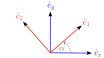
\includegraphics[scale = 0.7]{Figures/Base-Rotada.pdf}
    \caption{Base cartesiana $\hat{e}_x$ y $\hat{e}_y$ rotada en un ángulo $\alpha$ con respecto al eje $x$.}
    \label{fig:rotated-basis}
\end{figure}

Así, el vector $\vec{v}$ puede escribirse como
\begin{equation}
    \vec{v} = v_{1} \hat{e}_{1} + v_{2} \hat{e}_{2} = (v_1,v_2),
\end{equation}
donde $v_{1}, v_{2} \in \mathbb{R}$ son las componentes del vector $\vec{v}$ con respecto al conjunto $B' = \{\hat{e}_1,\hat{e}_2\}$. Los conjuntos $B$ y $B'$ son \textbf{bases} del espacio vectorial 2-dimensional $\mathbb{R}^2$, pero eso no es todo, son bases formadas por vectores ortonormales, es decir, 
\begin{align}
    \langle \hat{e}_{x}, \hat{e}_{y} \rangle &= 0, \quad  \langle \hat{e}_{x}, \hat{e}_{x} \rangle = \langle \hat{e}_{y}, \hat{e}_{y} \rangle = 1; \\
    \langle \hat{e}_{1}, \hat{e}_{2} \rangle &= 0, \quad  \langle \hat{e}_{1}, \hat{e}_{1} \rangle = \langle \hat{e}_{2}, \hat{e}_{2} \rangle = 1,
\end{align}
con $\langle , \rangle$ el \textbf{producto interno} (o \textbf{escalar}) usual en $\mathbb{R}^2$. Todo espacio vectorial con un producto interno definido se dice que es un \textbf{espacio pre-hilbert}.

Ahora bien, la vida no siempre es real, así que compliquemos la con los complejos. Consideremos el espacio vectorial complejo $\mathbb{C}^2$, todo vector $\vec{z}$ puede escribirse como combinación lineal de $\hat{e}_{1} = (1,0)$ y $\hat{e}_2 = (0,1)$ de tal forma que
\begin{equation}
    \vec{z} = z_{1} \hat{e}_{1} + z_{2} \hat{e}_{2} = (z_1,z_2),
\end{equation}
donde $z_{1}, z_{1} \in \mathbb{C}$ son las componentes del vector $\vec{z}$ con respecto al conjunto $\{\hat{e}_1,\hat{e}_2\}$. Además, en este espacio vectorial también podemos definir un producto interno. Sean $\vec{z} = (z_1,z_2) \in \mathbb{C}^2$ y $\vec{w} = (w_1,w_2) \in \mathbb{C}^2$, definimos
\begin{equation}
    \langle \vec{z}, \vec{w} \rangle := z_1 w_1^{*} + z_2 w_2^{*},
\end{equation}
donde $z^*$ es el complejo conjugado de $z$.

\begin{ejemplo}
    Dados los vectores $\vec{z} = (1,i)$ y $\vec{w} = (1 + 2i,i)$, tenemos que
    \begin{align}
      \langle \vec{z}, \vec{w} \rangle &= 1 \cdot (1 + 2i)^* + i \cdot (i)^* \nonumber \\
      &=  1 \cdot (1 - 2i) + i \cdot (-i) \nonumber \\
      &= 2 - 2i. 
    \end{align}
\end{ejemplo}

Los dos ejemplos anteriores son espacios de dimensión finita. Compliquemos el asunto considerando espacios de ¡dimensión infinita!... Pero nada muy extravagante, simplemente el espacio vectorial de funciones :). Recuerde de su curso de álgebra lineal que las funciones son vectores y forman un espacio vectorial. 

En particular, nos centraremos en el curso en el espacio formado por funciones seccionalmente continuas en el intervalo $[a,b]$ con imagen en el plano complejo, ésto es, funciones $f:[a,b] \rightarrow \mathbb{C}$. Denotaremos este conjunto por $\mathcal{PC}[a,b]$ \footnote{Debido a la palabra inglesa ``piecewise continuous".}. En cristiano, es el conjunto de las funciones continuas salvo en un número finito de puntos, pero la imagen de la función en los puntos de discontinuidad se encuentra acotada (no diverge), ver figura \ref{fig:fReal-PC} y \ref{fig:fComplex-PC}. Como se puede apreciar en la figura \ref{fig:fComplex-PC}, geométricamente, $f: [a,b] \longrightarrow \mathbb{C}$ es una curva en el plano complejo parametrizada por $t \in [a,b]$. 

\begin{figure}
    \centering
    \begin{subfigure}[t]{0.37\textwidth}
        \centering
        \includegraphics[width=\linewidth]{Figures/FuncionPC-1.pdf}
        \caption{Función real $f: [a,b] \rightarrow \mathbb{R}$ seccionalmente continua.}
        \label{fig:fReal-PC}
    \end{subfigure}\hskip 1em%
    \begin{subfigure}[t]{0.59\textwidth}
        \centering
        \includegraphics[width=\linewidth]{Figures/FuncionPC-2.pdf}
        \caption{Función compleja $f: [a,b] \rightarrow \mathbb{C}$ seccionalmente continua.}
        \label{fig:fComplex-PC}
    \end{subfigure}
\end{figure}

Al igual que en el caso de $\mathbb{R}^2$ y $\mathbb{C}^2$, podemos definir un producto interno en $\mathcal{PC}[a,b]$. Dadas dos funciones $f,g \in \mathcal{PC}[a,b]$, definimos el producto interno de $f$ y $g$ por 
\begin{shaded}
 \begin{equation}
    \langle f , g \rangle = \int_a^b f(x) g^*(x) \,dx. \label{eq:scalar-product}
\end{equation}   
\end{shaded}

Con la definición del producto interno, podemos saber cuando dos funciones son ortogonales (más aún ortonormales).  

\begin{ejemplo}
Considere el conjunto de funciones $c_n(x) \in \mathcal{PC}[-\pi,\pi]$ con $n = 0, \pm 1, \pm 2, \dots$, dadas por
\begin{equation}
c_n(x) = \frac{1}{\sqrt{2\pi}} e^{i nx}.   \label{eq:basis-exp} 
\end{equation}

Verifiquemos que forman un conjunto ortonormal. Para $n \neq m$, calculemos 
\begin{align}
    \langle c_n , c_m \rangle = \frac{1}{2\pi} \int_{-\pi}^{\pi} e^{i(n-m)x} \,dx &= \frac{1}{2\pi} \left[ -\frac{i}{n-m} e^{i(n-m) x}\right]_{-\pi}^{\pi} \nonumber \\
    &= \frac{i}{2\pi(m-n)} [e^{i n\pi} + e^{-i m \pi} - e^{-in \pi} - e^{im \pi}] \nonumber \\
    &= 0.
\end{align}

Por otro lado, para $n = m$, encontramos que 
\begin{equation}
  \langle c_n , c_n \rangle =\frac{1}{2\pi} \int_{-\pi}^{\pi} e^{i(n-n)x} \,dx = \frac{1}{2\pi} \int_{-\pi}^{\pi} 1 \,dx = 1.
\end{equation}

Por lo tanto,
\begin{equation}
\langle c_n , c_m \rangle = \delta_{nm}.    
\end{equation}

\end{ejemplo}

\begin{ejemplo}
Pruebe que el conjunto de funciones 
\begin{equation}
 \left\{ \frac{1}{\sqrt{2 \pi}}, \frac{\cos(nx)}{\sqrt{\pi}} ,  \frac{\sin(nx)}{\sqrt{\pi}} \right\}_{n=1}^{\infty} \label{eq:basis-trigono}  
\end{equation}
es ortonormal en $\mathcal{PC}[-\pi,\pi]$.
\end{ejemplo}

Los conjuntos \eqref{eq:basis-exp} y \eqref{eq:basis-trigono}, al ser ortogonales, son linealmente independientes, por tanto son candidatos a ser base para las funciones en el conjunto $\mathcal{PC}[-\pi,\pi]$. Más aún, para el conjunto de funciones seccionalmente continuas periódicas.

Nos faltaría probar que toda función periódica se puede escribir como combinación lineal de los conjuntos \eqref{eq:basis-exp} y \eqref{eq:basis-trigono}. Ésto es bastante complejo, requiere de la matemática del análisis funcional, pero el concepto clave es la completitud. Para ello, necesitamos una definición más formal:

\begin{defi}
Una sucesión de funciones $\{f_n\}_{n \in \mathbb{N}}$ en $\mathcal{PC}[a,b]$ se dice \textbf{sucesión de Cauchy} si dado $\varepsilon > 0$, existe un $N \in \mathbb{N}$ tal que
\begin{equation}
\forall n,m \geq N \quad \Rightarrow \quad \norm{f_n-f_m} < \varepsilon,    
\end{equation}
para cada $x \in [a,b]$, donde $\norm{f} := \sqrt{\langle f,f\rangle}$.
\end{defi}

Intuitivamente, los términos de la sucesión de funciones $\{f_{n}\}$ comienzan a acercarse la una a la otra, ver figura \ref{fig:Suc-Cauchy}.  Si las definiciones que usan $\epsilon-\delta$ les trae malos recuerdos, no se preocupe porque no se ocuparán, pero es relevante tener el concepto. 

\begin{figure}
    \centering
    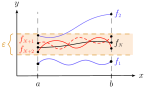
\includegraphics[scale = 0.65]{Figures/Sucesion-Cauchy.pdf}
    \caption{Representación gráfica de una sucesión de Cauchy.}
    \label{fig:Suc-Cauchy}
\end{figure}

Consideremos la combinación lineal de las funciones $\{\varphi_{n}\}$, es decir, la serie 
\begin{equation}
 \sum_{n = 1}^{\infty} c_n \varphi_n(x),
\end{equation}
en el espacio $\mathcal{PC}[a,b]$. Si toda sucesión de sumas parciales 
\begin{equation}
    S_n(x) = \sum_{k = 1}^{n} c_{n} \varphi_n(x)
\end{equation}
es de Cauchy y converge, entonces se dice que el espacio vectorial es \textbf{completo}. Si el espacio era pre-hilbert, como en el caso de $\mathcal{PC}[a,b]$, se dice que es de \textbf{Hilbert}, si además es completo.

\colorlet{shadecolor}{yellow!20}
\begin{shaded}
\vspace{0.1cm}
\textbf{Observación:} En Física se trabaja en un espacio más general que $\mathcal{PC}[a,b]$, el espacio de las funciones cuadrado integrables denotado por $\mathcal{L}^2[a,b]$. Este corresponde al espacio de funciones $f:[a,b] \rightarrow \mathbb{C}$, tales que 
\begin{equation}
\int_a^b |f(x)|^2 \,dx < \infty.    
\end{equation}

Por ejemplo, las funciones seccionalmente continuas son funciones cuadrado integrables.

El espacio $\mathcal{L}^2[a,b]$ es un espacio vectorial con producto interno definido por \eqref{eq:scalar-product} y la condición de cuadrado integrable es usada, por ejemplo, en mecánica cuántica, pues constituye la base para que el modulo al cuadrado de las funciones de onda tengan intepretación de densidades de probabilidad, según la interpretación de Copenhague (probabilística) de la mecánica cuántica.
\vspace{0.1cm}
\end{shaded}

La sucesión $\{f_{n}\}_{n\in \mathbb{N}}$ en el espacio $\mathcal{PC}[a,b]$ \textbf{converge en media} a una función $f$ si
\begin{equation}
    \lim_{n\to  \infty} \norm{f - \sum_{k=1}^{n} f_{{k}}} = \lim_{n\to \infty} \int_a^{b} \left[ f(x) - \sum_{k=1}^{n} f_{k}(x)\right]^2 dx = 0.
\end{equation}

Simbólicamente,
\begin{equation}
    f(x) \sim  \sum_{n=1}^{\infty} f_{n}(x).
\end{equation}

Es inmediato ver que 
\begin{equation}
    \text{$\{f_{n}\}$ converge en media a $f$} \Rightarrow \text{$\{f_{n}\}$ es de Cauchy.}
\end{equation}

Sin embargo, la convergencia en media no implica que la sucesión converge puntual o uniformente a $f$.

Si el conjunto de funciones $\{\varphi_{n}\}_{n\in \mathbb{N}}$  es tal que
\begin{equation}
     \lim_{n\to  \infty} \norm{f - \sum_{k=1}^{n} C_{k} \varphi_{k}} = 0,
\end{equation}
donde $C_{n}$ son las componentes de la combinación lineal de las funciones $\varphi_{n}$, decimos que $\{\varphi_{n}\}_{n\in \mathbb{N}}$ es un \textbf{conjunto completo}, pues al converger en media, es de Cauchy.

Si $\{\varphi_{n}\}_{n\in \mathbb{N}}$ son funciones ortogonales, entonces el conjunto $\{\varphi_{n}\}$ se dice ortogonal completo, o bien \textbf{base ortogonal} del espacio de funciones en cuestión, con $C_{n} =  \langle f, \varphi_{n}\rangle$.

\begin{ejemplo}
Los conjuntos
\begin{equation}
\left\{e^{i\frac{2\pi n}{T}x} \right\}_{n \in \mathbb{Z}} 
\end{equation}
y
\begin{equation}
 \left\{1, \cos\left(\frac{2\pi n}{T}x\right) ,  \sin\left(\frac{2\pi n}{T}x\right) \right\}_{n=1}^{\infty} \label{eq:basis-trigo}  
\end{equation}
son ortogonales completos respecto a $[0,T]$.
\end{ejemplo}

Si $f:[a,b] \longrightarrow \mathbb{C}$ se extiende periódicamente con período $T = b-a$ y definimos la \textbf{frecuencia fundamental} $\omega_1 := 2\pi/T$ y las \textbf{frecuencias armónicas} $\omega_n := n \omega_1, n = 0, \pm 1, \pm 2,\dots$. Entonces, la \textbf{serie de Fourier exponencial} puede escribirse como 
\colorlet{shadecolor}{green!20}
\begin{shaded}
\begin{equation}
 f(x) \sim \sum_{n = - \infty}^{\infty} f_n e^{i \omega_n x},  \label{eq:Fourier-Exp}  
\end{equation}
\end{shaded}
donde los coeficientes están dados por
\begin{equation}
 f_n = \frac{1}{T} \left\langle f, e^{i \omega_n x} \right\rangle = \frac{1}{T} \int_0^{T} f(x) e^{-i \omega_n x} \,dx, \quad n = 0, \pm 1, \pm 2, \dots   
\end{equation} 

Usando la identidad de Euler, se puede probar que la serie de Fourier exponencial para la función $f$ puede ser escrita en términos de las funciones trigonométricas seno y coseno como
\colorlet{shadecolor}{green!20}
\begin{shaded}
\begin{equation}
f(x) \sim \frac{a_0}{2} + \sum_{n=1}^{\infty} \left[a_n \cos(\omega_n x) + b_n \sin(\omega_n x) \right], \label{eq:Fourier-Trigo}       
\end{equation}
\end{shaded}
donde
 \begin{align}
    a_0 &= \frac{2}{T} \left\langle f, 1 \right\rangle = \frac{2}{T} \int_0^{T} f(x) \,dx , \\
    a_n &= \frac{2}{T}\langle f,\cos(\omega_{n} x) \rangle = \frac{2}{T} \int_0^{T} f(x) \cos(\omega_n x) \,dx; \quad n = 1,2 \dots \\
    b_n &=\frac{2}{T}\langle f,\sin(\omega_{n} x) \rangle =\frac{2}{T} \int_0^{T} f(x) \sin(\omega_n x) \,dx; \quad n = 1,2 \dots
\end{align}   

Los coeficientes de las series \eqref{eq:Fourier-Exp} y \eqref{eq:Fourier-Trigo} están relacionados por 
\begin{equation}
a_0 = 2c_0,\quad a_n = c_n + c_{-n}, \quad b_n = i(c_n - c_{-n}); \quad n = 1,2, \dots,  
\end{equation}
o bien, 
\begin{equation}
    c_n = \left\{ \begin{array}{cl}
        \frac{1}{2} (a_n - ib_n), & n \geq 0  \\
    \frac{1}{2}(a_{-n} + i b_{-n}),     & n  \leq -1 
    \end{array} \right. . 
\end{equation}

Antes de terminar este repaso, es importante destacar que la serie de Fourier de una función $f(x)$ seccionalmente continua no converge necesariamente de forma puntual a la función $f(x)$. Por ejemplo, si consideramos la función signo definida por
\begin{equation}
 f(x) := \left\{ \begin{array}{cc}
     -1,& - \pi \leq x < 0  \\
     1,&   0 \leq x \leq \pi
\end{array} \right.,  
\end{equation}
puede demostrarse que su serie de Fourier es 
\begin{equation}
 f(x) = \sum_{k=1}^{\infty} \frac{4}{\pi} \frac{\sin[(2k-1)x]}{(2k-1)}.   
\end{equation}

Notemos que la serie de Fourier de $f$ para todo $x\in \mathbb{R}$ representa la extensión periódica de los valores de $f(x)$ en el intervalo $[-\pi,\pi]$ y que a pesar de haber escrito que la función $f$ es igual a la serie, debemos tener en cuenta que en los punto $x = 0$ y $x = \pm \pi$ converge al valor medio del salto de la discontinuidad, ver figura \ref{fig:EjemploFourier2}

\begin{figure}[H]
    \centering
    \includegraphics[scale = 0.65]{Figures/EjemploFourier2.pdf}
    \caption{Serie de Fourier de la función signo truncada hasta $n = 4$.}
     \label{fig:EjemploFourier2}
\end{figure}


En general, se tiene el siguiente teorema.

\begin{teorema}[Convergencia puntual de la serie de Fourier] \label{Puntual}
Sea $f(x)$ una función periódica (o extensión periódica) seccionalmente continua, tenemos que
\begin{equation}
    \sum_{n = - \infty}^{\infty} f_n e^{i \omega_n x} = \lim_{\varepsilon \to 0^{+}} \frac{f(x + \varepsilon) - f(x - \varepsilon)}{2},
\end{equation}
\vspace{-0.05cm}
para cada $x \in \mathbb{R}$, donde ambas derivadas laterales $f'(x^+)$ y $f'(x^-)$ existen.
\end{teorema}

Note que en los puntos donde $f$ es continua,
\begin{equation}
    f(x) = \sum_{n = - \infty}^{\infty} f_n e^{i \omega_n x}.
\end{equation}

En la figura \ref{fig:Fourier-Domains} está representada la descomposición en serie de Fourier de un pulso cuadrado, siendo éste descrito por la superposición de funciones sinusoidales en el dominio temporal (gráfica de la izquierda). Por otro lado, en la gráfica de la derecha, están graficadas las amplitudes de cada una las funciones sinusoidales de la descomposición en Fourier en función de su frecuencia. Note que la serie de Fourier nos permite pasar de un dominio continuo (el temporal), a uno discreto (el de frecuencias).

\begin{figure}
    \centering
    \includegraphics[scale = 0.9]{Figures/Fourier-Dominios.pdf}
    \caption{Serie de Fourier de un pulso cuadrado en el dominio temporal $t$ y en el dominio de las frecuencias $\omega_{n}/2\pi$ adaptado de \href{https://tikz.net/fourier_series/}{tikz.net}.}
    \label{fig:Fourier-Domains}
\end{figure}

\section{Transformada de Fourier}

Sea $f:\mathbb{R} \rightarrow \mathbb{C}$, la \textbf{transformada de Fourier} de $f$ se encuentra definida por
\begin{shaded}
\begin{equation}
    \mathcal{F}\{f(x)\}(\omega) \equiv \hat{f}(\omega) := \frac{1}{\sqrt{2\pi}} \int_{-\infty}^{+\infty} f(x) e^{-i\omega x} dx, \label{eq:Fourier-Trans}
\end{equation}    
\end{shaded}
\noindent y la \textbf{transformada inversa} por 
\begin{shaded}
\begin{equation}
 \mathcal{F}^{-1}\{\hat{f}(\omega)\} (x) := \frac{1}{\sqrt{2\pi}} \int_{-\infty}^{+\infty} \hat{f}(\omega) e^{i\omega x} d\omega.   \label{eq:Fourier-Inv}
\end{equation}    
\end{shaded}

La transformada de Fourier es la extensión natural del concepto de series de Fourier para funciones no periódicas. Además, al ser $n$ una variable discreta, y $\omega$ continua, podemos decir que la transformada de Fourier es la generalización del concepto de series de Fourier cuando las funciones pertenecen a un espacio vectorial de dimensión infinita pero continua.

\colorlet{shadecolor}{yellow!20}
\begin{shaded}
\vspace{0.1cm}
\textbf{Observación:}
\begin{itemize}
\item El factor $1/\sqrt{2\pi}$ en la definición \eqref{eq:Fourier-Trans} es hasta cierto punto convencional. Lo importante es que se cumpla la identidad
    \begin{equation}
        f(x) \sim \frac{1}{2\pi} \int_{-\infty}^{\infty} \left[\int_{-\infty}^{\infty} f(\xi) e^{-i\omega\xi} d\xi \right] e^{i\omega x} \,d\omega.
      \label{IntegralFourier}
    \end{equation}
   
    Por ejemplo, en lugar de estos factores, podríamos tener un factor $\alpha$ en \eqref{eq:Fourier-Inv} y $1/(2\pi \alpha)$ en \eqref{eq:Fourier-Trans}, con $\alpha$ una constante arbitraria. Algunas elecciones populares son: $\alpha = 1$ y $\alpha = 1/\sqrt{2\pi}$ \cite{Rubilar}.

    \item Al igual que el factor $1/\sqrt{2\pi}$ en la definición \eqref{eq:Fourier-Trans}, la función $e^{-i\omega x}$ es convencional y puede ser reemplazada por $e^{i\omega x}$, siempre y cuando se verifique \eqref{IntegralFourier} \cite{Butkov, Riley}.
    
    \item En 3 dimensiones, la integral de Fourier está dada por:
    \begin{align*}
         f(\vec{r}\,) &:= \int_{\mathbb{R}^3} \tilde{f}(\vec{k}) e^{i (\vec{k} \cdot \vec{r})} d^3k, \\
         \tilde{f}(\vec{k}\,) &:= \frac{1}{(2\pi)^3} \int_{\mathbb{R}^3} f(\vec{r}) e^{-i (\vec{k} \cdot \vec{r})} d^3x,
    \end{align*}
    donde $\vec{k}$ es el vector de onda jugando el papel de la frecuencia, pero espacial.
    
    En general, en $n$ dimensiones:
     \begin{align*}
         f(\vec{r}\,) &:= \int_{\mathbb{R}^n} \tilde{f}(\vec{k}) e^{i (\vec{k} \cdot \vec{r})} d^n k, \\
         \tilde{f}(\vec{k}\,) &:= \frac{1}{(2\pi)^n} \int_{\mathbb{R}^n} f(\vec{r}) e^{-i (\vec{k} \cdot \vec{r})} d^n x.
    \end{align*}

\end{itemize}
\end{shaded}

Si la función $f(x)$ es \textbf{absolutamente integrable}, es decir,
\begin{equation}
    \int_{-\infty}^{\infty} |f(x)| \,dx < \infty,
\end{equation}
la transformada de Fourier existe. Sin embargo, la condición de que $f$ sea absolutamente integrable es suficiente pero no necesaria para la existencia de la transformada de Fourier. 

Similar a la serie de Fourier, en estricto rigor, la transformada inversa de Fourier no converge a la función $f$. En general, se tiene el siguiente teorema.

\begin{teorema}[Convergencia de la transformada inversa de Fourier] 
Sea $f(x)$ una función seccionalmente continua en cada intervalo finito del eje $x$, y  supongamos que es absolutamente integrable en $(-\infty, + \infty)$. Entonces,
\begin{equation}
    \frac{1}{\sqrt{2\pi}} \int_{-\infty}^{+\infty} \hat{f}(\omega) e^{i\omega x} d\omega. = \lim_{\varepsilon \to 0^{+}} \frac{f(x + \varepsilon) - f(x - \varepsilon)}{2},
\end{equation}
\vspace{-0.05cm}
para cada $x \in \mathbb{R}$, donde ambas derivadas laterales $f'(x^+)$ y $f'(x^-)$ existen.
\end{teorema}

En los puntos donde $f$ es continua,
\begin{equation}
    f(x) = \frac{1}{\sqrt{2\pi}} \int_{-\infty}^{+\infty} \hat{f}(\omega) e^{i\omega x} d\omega.
\end{equation}

\begin{ejemplo}[Pulso cuadrado] \label{PulsoCuadrado}
Consideremos la función 
\begin{equation}
f(x) = \left\{ \begin{array}{cl}
     1,& |x|<a  \\
     0,& |x|> a
\end{array} \right..   
\end{equation}

Su transformada de Fourier está dada por
\begin{align}
    \hat{f}(\omega) &= \frac{1}{\sqrt{2\pi}} \int_{-\infty}^{\infty} f(x) e^{-i\omega x} dx \nonumber \\
    &= \frac{1}{\sqrt{2\pi}} \int_{-a}^a (1)  e^{-i\omega x} dx \nonumber \\
    &= \frac{1}{\sqrt{2\pi}} \left[ - \frac{1}{i\omega} e^{-i\omega x} \right]_{-a}^a \nonumber\\
    &= \frac{1}{\sqrt{2\pi} \omega i} [e^{i\omega a} - e^{-i\omega a}] \nonumber\\
    &= \sqrt{\frac{2}{\pi}} \frac{\sin(\omega a)}{\omega}. \label{eq:TransPulsoCuadrado}
\end{align}

\begin{figure}[H]
    \centering
    \includegraphics[scale = 0.59]{Figures/EjemploTransformada1.pdf}
    \caption{Pulso cuadrado y su transformada de Fourier, con $a = 5$.}
    \label{Espectro2}
\end{figure}
\end{ejemplo}

\begin{ejemplo}[Distribución gaussiana]

Considere la gaussiana
\begin{equation}
f(x) = n e^{-\alpha x^2}, \quad  \alpha > 0.    
\end{equation}

Su transformada de Fourier está dada por 
\begin{equation}
    \hat{f}(\omega) =  \frac{n}{\sqrt{2\pi}} \int_{-\infty}^{\infty} e^{-\alpha x^2} e^{-i\omega x} dx =  \frac{n}{\sqrt{2\pi}} \int_{-\infty}^{\infty} e^{-\alpha x^2-i\omega x} dx . \label{eq:Gauss-Fourier-1}
\end{equation}

Notemos que 
\begin{align}
    -\alpha x^2-i\omega x &= - \alpha \left( x^2 + \frac{i\omega}{\alpha}x \right) \nonumber\\
    &= - \alpha \left( x^2 + \frac{i\omega}{\alpha} x + \left( \frac{i\omega}{2\alpha} \right)^2 - \left( \frac{i\omega}{2\alpha} \right)^2 \right) \nonumber \\
    &= - \alpha \left( x + \frac{i\omega}{2\alpha} \right)^2 + \alpha \left( \frac{i\omega}{2\alpha} \right)^2 \nonumber \\
    &= - \alpha \left( x + \frac{i\omega}{2\alpha} \right)^2 - \left( \frac{\omega^2}{4\alpha} \right).  \label{eq:Gauss-Fourier-2}
\end{align}

Reemplazando la ecuación \eqref{eq:Gauss-Fourier-2} en \eqref{eq:Gauss-Fourier-1}, podemos escribir
\begin{equation}
    \hat{f}(\omega) =  \frac{n}{\sqrt{2\pi}} \int_{-\infty}^{\infty} e^{-\alpha \left( x + \frac{i\omega}{2\alpha} \right)^2 - \left( \frac{\omega^2}{4\alpha} \right)}  dx = \frac{n}{\sqrt{2\pi}} e^{- \left( \frac{\omega^2}{4\alpha} \right)} \int_{-\infty}^{\infty} e^{-\alpha \left( x + \frac{i\omega}{2\alpha} \right)^2} \,dx. 
\end{equation}

Haciendo el cambio de variable $u = x + \frac{i\omega}{2\alpha}$, obtenemos que \footnote{}
\begin{equation}
    \hat{f}(\omega) = \frac{n}{\sqrt{2\pi}} e^{- \left( \frac{\omega^2}{4\alpha} \right)} \int_{-\infty}^{\infty} e^{-\alpha u^2} \,du.
\end{equation}

Como
\begin{equation}
\int_{-\infty}^{\infty} e^{-\alpha x^2} \,dx = \sqrt{\frac{\pi}{\alpha}}, \quad \alpha > 0,    
\end{equation} 
obtenemos que 
\begin{equation}
\hat{f}(\omega) = \frac{n}{\sqrt{2\alpha}} e^{- \left( \frac{\omega^2}{4\alpha} \right)}.  \label{eq:Fourier-Gaussiana}  
\end{equation}
\vfill
    \footnoterule
    
    {\footnotesize
    $^2$ En estricto rigor se debería calcular una integral compleja, vea \cite{Arfken}.
    }

\begin{figure}[H]
    \centering
    \includegraphics[scale = 0.6]{Figures/EjemploTransformada2.pdf}
    \caption{Distribución gaussiana y su transformada de Fourier para $n=1$ y $\alpha =1$ .}
    \label{Espectro3}
\end{figure}

\begin{figure}[H]
    \centering
    \includegraphics[scale = 0.6]{Figures/EjemploTransformada3.pdf}
    \caption{Distribución gaussiana y su transformada de Fourier para $n=1$ y $\alpha =0.25$ .}
    \label{Espectro4}
\end{figure}
\end{ejemplo}

\subsection{Propiedades de la Transformada de Fourier}

Sean $f$ y $g$ dos funciones absolutamente integrables, y $\alpha,\beta \in \mathbb{C}$, la transformada de Fourier verifica las siguientes propiedades:
\begin{enumerate}
    \item \textbf{Linealidad:} 
    \begin{equation}
        \mathcal{F}\{\alpha f + \beta g\}(\omega) = \alpha \mathcal{F}\{f\}(\omega) + \beta \mathcal{F}\{g\}(\omega). 
    \end{equation}

\item Si $f$ es real, entonces
\begin{equation}
    \mathcal{F}\{f\}(-\omega) = [\hat{f}(\omega)]^{*}.
\end{equation}

\item \textbf{Traslación y cambio de escala:} Si $a,b\in \mathbb{R}$, entonces
\begin{equation}
    \mathcal{F}\{f(ax + b)\}(\omega) = \frac{1}{|a|} e^{i\frac{b}{a}\omega} \hat{f}\left( \frac{\omega}{a}\right), \qquad a \neq 0. \label{eq:Traslation-Fourier}
\end{equation}

\item \textbf{Multiplicación por la exponencial compleja:} 
\begin{equation}
    \mathcal{F}\{e^{\alpha x} f(x)\}(\omega) = \hat{f}(\omega + i \alpha).
\end{equation}

\item \textbf{Transformada de la derivada:} Si $\lim\limits_{x\to \pm\infty} f(x) = 0$, entonces
\begin{equation}
    \mathcal{F}\{f^{(n)}\}(\omega) = (i \omega)^{n} \hat{f}(\omega). \label{eq:Dev-Fourier}
\end{equation}
\end{enumerate}

En el contexto de las transformadas de funciones, resulta conveniente definir una nueva operación, la \textbf{convolución}. Dadas dos funciones reales $f(x)$ y $g(x)$, se define la  \textit{convolución} de las funciones $f$ y $g$ como 
\colorlet{shadecolor}{green!20}
\begin{shaded}
\begin{equation}
 (f*g)(x) := \int_{-\infty}^{\infty} f(v) g(x-v) \,dv.   \label{eq:Convolucion}
\end{equation}    
\end{shaded}

Aunque no lo crea, ya se ha encontrado anteriormente con esta operación en Electromagnetismo. Por ejemplo, el potencial electrostático debido a una densidad de carga $\rho(\Vec{x})$ se puede escribir como
\begin{equation}
\phi(\Vec{x}) = \int_{V} \frac{\rho(\Vec{x}\,')}{|\Vec{x} - \Vec{x}\,'|} \, dV' = (\rho * f)(\Vec{x}),    
\end{equation}
donde  $f(\Vec{x}) = 1/|\Vec{x}|$.

\begin{figure}[H]
    \centering
    \includegraphics[scale = 0.55]{Figures/Distribucion-Cargas.pdf}
    \caption{Distribución de carga de densidad $\rho(\Vec{x})$.}
    \label{fig:PotencialDistribucion}
\end{figure}

La convolución es conmutativa, asociativa y verifica la distributividad con respecto a la suma. Además, la transformada de Fourier de la convolución es
\begin{shaded}
    \begin{equation}
        \mathcal{F}\{f*g\}(\omega) = \sqrt{2\pi} \hat{f}(\omega) \hat{g}(\omega). \label{eq:convolution-teo-1}
    \end{equation}
\end{shaded}

Si tomamos la transformada inversa, obtenemos el siguiente importante resultado:
\begin{shaded}
    \begin{equation}
        (f*g)(x) = \sqrt{2\pi} \mathcal{F}^{-1}\{\hat{f}(\omega) \hat{g}(\omega)\}(x). \label{eq:convolution-teo-2}
    \end{equation}
\end{shaded}

En lo anterior yace la importancia práctica de la convolución: la transformada inversa del producto de dos transformadas de Fourier es la convolución.

Usando \eqref{eq:convolution-teo-2}, puede demostrarse la  \textbf{identidad de Parseval}:
\begin{shaded}
\begin{equation}
        \int_{-\infty}^{\infty} |f(x)|^2 \,dx =  \int_{-\infty}^{\infty} |\hat{f}(\omega)|^2 \,d\omega.
    \end{equation}    
\end{shaded}

\begin{ejemplo}
    Use el teorema de Parseval para evaluar
    \begin{equation}
      \int_{-\infty}^{\infty}  \frac{\sin^2(x)}{x^2} \,dx.
    \end{equation}

    \textbf{Solución:} Esta integral puede ser calculada usando el teorema del residuo. En nuestro caso, usaremos la identidad de Parseval, teniendo en cuenta el resultado de la transformada de Fourier del pulso cuadrado en el ejemplo \ref{PulsoCuadrado}. 

    Tomando $a = 1$ en la ecuación \eqref{eq:TransPulsoCuadrado}, obtenemos que
    \begin{equation}
     \int_{- \infty}^{\infty} |\hat{f}(\omega)|^2 \,d\omega = \int_{- \infty}^{\infty} \frac{2}{\pi}\frac{\sin^2(\omega)}{\omega^2}  \,d\omega = \frac{2}{\pi} \int_{-\infty}^{\infty}  \frac{\sin^2(\omega)}{\omega^2} \,d\omega.   
    \end{equation}

    Usando la identidad de Parseval, encontramos
    \begin{align}
        \int_{- \infty}^{\infty} |\hat{f}(\omega)|^2 \,d\omega &= \int_{-\infty}^{\infty} |f(x)|^2 \,dx \\
        \Rightarrow \frac{2}{\pi} \int_{-\infty}^{\infty}  \frac{\sin^2(\omega)}{\omega^2} \,d\omega &=  \int_{-1}^1  \,dx = 2. 
    \end{align}

Por lo tanto,
\begin{equation}
\int_{-\infty}^{\infty}  \frac{\sin^2(\omega)}{\omega^2} \,dk = \pi. 
\end{equation}

\end{ejemplo}


\section{Transformada de Fourier de funciones con simetría}

Recordemos que si $f$ es una función par,
\begin{equation}
    \int_{-L}^{L} f(x) \,dx = 2 \int_{0}^{L} f(x) \,dx,
\end{equation}
y si $f$ es impar,
\begin{equation}
    \int_{-L}^{L} f(x) \,dx = 0.
\end{equation}

Consideremos la función $f(x)$ real e impar, entonces
\begin{align}
    \hat{f}(\omega) &= \frac{1}{\sqrt{2\pi}} \int_{-\infty}^{\infty} f(x) e^{-i\omega x} dx \nonumber \\
&= \frac{1}{\sqrt{2\pi}} \int_{-\infty}^{\infty} f(x) [\cos(\omega x) - i \sin(\omega x)] \,dx \nonumber \\
 &= \frac{1}{\sqrt{2\pi}} \cancelto{0}{\int_{-\infty}^{\infty} f(x) \cos(\omega x) \,dx}  - \frac{i}{\sqrt{2\pi}} \int_{-\infty}^{\infty} f(x) \sin(\omega x) \, dx \nonumber \\
     &= - \frac{2i}{\sqrt{2\pi}} \int_{0}^{\infty} f(x) \sin(\omega x) \, dx \nonumber \\
     &= - i \sqrt{\frac{2}{\pi}} \int_{0}^{\infty} f(x) \sin(\omega x) \,dx \equiv - i  \hat{f}_{\rm S}(\omega), 
\end{align}
donde $\hat{f}_{\rm S}$ es conocida como la \textbf{transformada seno de Fourier} de la función $f(x)$, y viene definida por \cite{Mauch} 
\begin{shaded}
    \begin{equation}
        \hat{f}_{\rm S}(\omega) := \sqrt{\frac{2}{\pi}} \int_{0}^{\infty} f(x) \sin(\omega x) \,dx.
    \end{equation}
\end{shaded}

Note además que $\hat{f}(-\omega) = - \hat{f}(\omega)$, es decir, la transformada de Fourier de una función impar es impar. 

Por otro lado, la transformada inversa nos queda
\begin{align}
    \mathcal{F}^{-1}\{\hat{f}(\omega)\}(x)  &= \frac{1}{\sqrt{2\pi}} \int_{-\infty}^{\infty} \hat{f}(\omega) e^{i\omega x} d\omega \nonumber \\
&= \frac{1}{\sqrt{2\pi}} \int_{-\infty}^{\infty} \hat{f}(\omega) [\cos(\omega x) + i \sin(\omega x)] \,d\omega \nonumber \\
 &= \frac{1}{\sqrt{2\pi}} \cancelto{0}{\int_{-\infty}^{\infty} \hat{f}(\omega) \cos(\omega x) \,d\omega}  + \frac{i}{\sqrt{2\pi}} \int_{-\infty}^{\infty} \hat{f}(\omega) \sin(\omega x) \, d\omega \nonumber \\
     &= \frac{2i}{\sqrt{2\pi}} \int_{0}^{\infty} \hat{f}(\omega) \sin(\omega x) \, d\omega \nonumber \\
     &= \sqrt{\frac{2}{\pi}} \int_{0}^{\infty} \hat{f}_{\rm S}(\omega) \sin(\omega x) \,d\omega. 
\end{align}

Así, definimos la \textbf{transformada inversa seno de Fourier} como
\begin{shaded}
    \begin{equation}
         \mathcal{F}^{-1}_{\rm S}\{\hat{f}(\omega)\}(x) = \sqrt{\frac{2}{\pi}} \int_{0}^{\infty} \hat{f}_{\rm S}(\omega) \sin(\omega x) \,d\omega. 
    \end{equation}
\end{shaded}

Análogamente a la definición de la  transformada seno de Fourier, si $f(x)$ es real y par, entonces 
\begin{align}
    \hat{f}(\omega) &= \frac{1}{\sqrt{2\pi}} \int_{-\infty}^{\infty} f(x) e^{-i\omega x} dx \nonumber \\
&= \frac{1}{\sqrt{2\pi}} \int_{-\infty}^{\infty} f(x) [\cos(\omega x) - i \sin(\omega x)] \,dx \nonumber \\
 &= \frac{1}{\sqrt{2\pi}} \int_{-\infty}^{\infty} f(x) \cos(\omega x) \,dx  - \frac{i}{\sqrt{2\pi}} \cancelto{0}{\int_{-\infty}^{\infty} f(x) \sin(\omega x) \, dx} \nonumber \\
     &=  \frac{2}{\sqrt{2\pi}} \int_{0}^{\infty} f(x) \cos(\omega x) \, dx \nonumber \\
     &= \sqrt{\frac{2}{\pi}} \int_{0}^{\infty} f(x) \cos(\omega x) \,dx \equiv  \hat{f}_{\rm C}(\omega), 
\end{align}
donde $\hat{f}_{\rm C}$ es conocida como la \textbf{transformada coseno de Fourier} de la función $f(x)$, y viene definida por \cite{Mauch} 
\begin{shaded}
    \begin{equation}
        \hat{f}_{\rm C}(\omega) := \sqrt{\frac{2}{\pi}} \int_{0}^{\infty} f(x) \cos(\omega x) \,dx. \label{eq:Fourier-Cos}
    \end{equation}
\end{shaded}

Note además que $\hat{f}(-\omega) = \hat{f}(\omega)$, es decir, la transformada de Fourier de una función par es par. 

Por otro lado, la transformada inversa nos queda
\begin{align}
    \mathcal{F}^{-1}\{\hat{f}(\omega)\}(x)  &= \frac{1}{\sqrt{2\pi}} \int_{-\infty}^{\infty} \hat{f}(\omega) e^{i\omega x} d\omega \nonumber \\
&= \frac{1}{\sqrt{2\pi}} \int_{-\infty}^{\infty} \hat{f}(\omega) [\cos(\omega x) + i \sin(\omega x)] \,d\omega \nonumber \\
 &= \frac{1}{\sqrt{2\pi}} \int_{-\infty}^{\infty} \hat{f}(\omega) \cos(\omega x) \,d\omega  + \frac{i}{\sqrt{2\pi}} \cancelto{0}{\int_{-\infty}^{\infty} \hat{f}(\omega) \sin(\omega x) \, d\omega} \nonumber \\
     &= \frac{2}{\sqrt{2\pi}} \int_{0}^{\infty} \hat{f}(\omega) \cos(\omega x) \, d\omega \nonumber \\
     &= \sqrt{\frac{2}{\pi}} \int_{0}^{\infty} \hat{f}_{\rm C}(\omega) \cos(\omega x) \,d\omega. 
\end{align}

Así, definimos la \textbf{transformada inversa coseno de Fourier} como
\begin{shaded}
    \begin{equation}
         \mathcal{F}^{-1}_{\rm C}\{\hat{f}(\omega)\}(x) = \sqrt{\frac{2}{\pi}} \int_{0}^{\infty} \hat{f}_{\rm C}(\omega) \cos(\omega x) \,d\omega. 
    \end{equation}
\end{shaded}

\begin{ejemplo}[Listado 1 - Problema 6]
    La función
\begin{equation}
    f(x) = \left\{ \begin{array}{cl}
        1, & \text{si $|x| < 1$}  \\
        0, & \text{si $|x| > 1$}
    \end{array} \right.
\end{equation}
es una función barrera finita simétrica.

\textbf{(a)} Encontrar la transformada coseno de Fourier $\hat{f}_{\rm C}(\omega)$.

\textbf{Solución:} La función $f$ es par, entonces su transformada de Fourier coincide con la transformada coseno de Fourier. Así, usando la definición \eqref{eq:Fourier-Cos}, obtenemos que
\begin{align}
    \hat{f}_{\rm C}(\omega) &= \sqrt{\frac{2}{\pi}} \int_0^{\infty}f(x) \cos(\omega x) \,dx \nonumber\\
    &= \sqrt{\frac{2}{\pi}} \int_{0}^{1} \cos(\omega x) \,dx \nonumber \\
    &= \left. \sqrt{\frac{2}{\pi}} \frac{\sin(\omega x)}{\omega} \right|_{0}^{1} \nonumber \\
    &= \sqrt{\frac{2}{\pi}} \frac{\sin(\omega)}{\omega}.
\end{align}

Por lo tanto,
\begin{equation}
    \hat{f}_{\rm C}(\omega) = \sqrt{\frac{2}{\pi}} \frac{\sin(\omega)}{\omega}.
\end{equation}

\textbf{(b)} Tomando la transformada coseno de Fourier inversa, mostrar que 
\begin{equation}
    f(x) = \frac{2}{\pi} \int_{0}^{\infty} \frac{\sin(\omega) \cos(\omega x)}{\omega} d\omega.
\end{equation}

\textbf{Solución:} La transformada coseno de Fourier inversa está dada por
\begin{align}
    \mathcal{F}^{-1}_{\rm C}\{\hat{f}_{\rm C}(\omega)\}(x) &= \sqrt{\frac{2}{\pi}} \int_{0}^{\infty} \hat{f}_{\rm C}(\omega) \cos(\omega x) \,d\omega \\
    &= \frac{2}{\pi} \int_{0}^{\infty} \frac{\sin(\omega) \cos(\omega x)}{\omega} d\omega. \label{eq:sign-funcion-inv}
\end{align}

Como la transformada coseno de Fourier inversa, coincide con la transformada inversa normal y $f$ es una función continua , podemos concluir que
\begin{equation}
    f(x) = \frac{2}{\pi} \int_{0}^{\infty} \frac{\sin(\omega) \cos(\omega x)}{\omega} d\omega.
\end{equation}

Si en verdad queremos probar que \eqref{eq:sign-funcion-inv} da la función $f(x)$, escribamos
\begin{align}
    \frac{\sin(\omega)\cos(\omega x)}{\omega} &= \frac{1}{\omega} \left( \frac{e^{i\omega} - e^{-i\omega}}{2i}\right) \left( \frac{e^{i\omega x} + e^{-i\omega x}}{2}\right) \nonumber\\
    &= \frac{1}{4i\omega} \left(e^{i\omega(x + 1)} + e^{-i\omega(x-1)} - e^{i\omega(x-1)} - e^{-i\omega(x+1)} \right) \nonumber\\
    &= \frac{2i}{4i\omega} \left[ \left( \frac{e^{i\omega(x+1)} - e^{-i\omega(x+1)}}{2i}\right)  - \left( \frac{e^{i\omega(x-1)} - e^{-i\omega(x-1)}}{2i}\right)\right] \nonumber\\
    &= \frac{1}{2\omega} \left\{\sin[\omega(x+1)] - \sin[\omega(x-1)]\right\}.
\end{align}

Por lo tanto, debemos calcular
\begin{equation}
     \mathcal{F}^{-1}_{\rm C}\{\hat{f}_{\rm C}(\omega)\}(x) = \frac{1}{\pi} \int_{0}^{\infty} \left\{\frac{\sin[\omega(x+1)]}{\omega} - \frac{\sin[\omega(x-1)]}{\omega}\right\} \,d \omega. \label{eq:Inv-Sign}
\end{equation}

En el apéndice (-), encontramos que \footnote{}
\begin{equation}
    \int_{0}^{\infty} \frac{\sin(\alpha \omega)}{\omega} d\omega = \left\{ \begin{array}{cl}
        \pi/2, & \text{si $\alpha > 0$}  \\
        0, & \text{si $\alpha = 0$} \\
        -\pi/2, & \text{si $\alpha < 0$}
    \end{array} \right. .
\end{equation}

Entonces, la ecuación \eqref{eq:Inv-Sign} nos queda
\begin{align}
    \mathcal{F}^{-1}_{\rm C}\{\hat{f}_{\rm C}(\omega)\}(x) &= \frac{1}{\pi} \left\{ \begin{array}{cl}
        - \pi/2 + \pi/2, & \text{si $x < -1$} \\
        \pi/2 - \left( - \pi/2 \right), & \text{si $-1 < x < 1$} \\
        \pi/2 - \pi/2, & \text{si $x > 1$}
    \end{array}\right. \nonumber \\
    &= \left\{ \begin{array}{cl}
        0, & \text{si $x < -1$} \\
        1, & \text{si $-1 < x < 1$} \\
        0, & \text{si $x > 1$}
    \end{array}\right. \nonumber \\
    &= f(x).
\end{align}

\vfill
    \footnoterule
    
    {\footnotesize
    $^3$ Puede convencerse con \textit{Wolframalpha} o su calculadora de integrales favorita.
    }

\end{ejemplo}

\section{Delta de Dirac}

La ``función" \textbf{delta de Dirac} $\delta(x)$ se encuentra definida por
\begin{equation}
\delta(x-a) = \left\{ \begin{array}{cl}
    0, & \text{si $x \neq a$}  \\
    \infty, & \text{si $x = a$} 
\end{array} \right.,    
\end{equation}
tal que la integral de $\delta(x)$ está normalizada a uno:
\begin{equation}
\int_{-\infty}^{\infty} \delta(x-a) \,dx = 1    
\end{equation}
y que satisface la propiedad
\begin{equation}
  \int_{-\infty}^{\infty} \delta(x-a) f(x) \,dx = f(a),
\end{equation}
para toda $f(x)$ continua.

Vemos que $\delta(x)$ puede ser infinitamente alta. Sin embargo, en el usual sentido de función, $\delta(x)$ no existe. No obstante, existen sucesiones de funciones las cuales se acercan a las propiedades de $\delta(x)$ ya mencionadas. Por ejemplo, las sucesiones de funciones \footnote{En el siguiente programa de \href{https://www.geogebra.org/m/snk6hnus}{Geogebra} encontrará una animación de las sucesiones de funciones discutidas.}
\begin{align}
    \phi_n(x) &= \frac{n}{\pi} \frac{1}{1+n^2 x^2}, \\
     \phi_n(x) &= \frac{n}{\sqrt{\pi}} e^{-n^2x^2},\\
      \phi_n(x) &=  \frac{1}{n\pi} \frac{\sin^2(nx)}{x^2},
\end{align}
en el límite $n \to \infty$, tienden a una delta de Dirac, están normalizadas a uno, 
\begin{equation}
  \int_{-\infty}^{\infty} \phi_n(x) \,dx = 1,  
\end{equation}
y para $f(x)$ continua, se verifica que 
\begin{equation}
  \lim_{n \to \infty} \int_{-\infty}^{\infty} \phi_n(x) f(x) \,dx = f(0).  
\end{equation}

Pero de nuevo, es incorrecto decir que estas sucesiones \textit{convergen} a la función $\delta$: los límites de esas sucesiones no existen. \footnote{Lo expuesto anteriormente se encuentra resumido en el siguiente \href{https://www.instagram.com/reel/C0mIjYotIOZ/?utm_source=ig_web_copy_link&igsh=MzRlODBiNWFlZA==}{Reel}.}

\colorlet{shadecolor}{yellow!20}
\begin{shaded}
\vspace{0.1cm}
\textbf{Nota:} La función delta fue introducida por el físico Paul Dirac, la cual tiene aplicaciones en mecánica cuántica, en el modelamiento de masas puntuales e impulsos instantáneos. Por ejemplo, considere un sistema compuesto por una masa unida a un resorte. Si el sistema es perturbado por una fuerza de impulso $I$ en el instante $t = 0$, la ecuación de movimiento es
\begin{equation}
    m \frac{d^2 x}{dt^2} + k x = I\delta(t),
\end{equation}
donde $m$ es la masa, $x$ el estiramiento del resorte con respecto a la posición de equilibrio, y $k$ es la constante del resorte.

Es llamada función delta porque es el análogo continuo a la delta de Kronecker. El rigor matemático de la función delta fue desarrollado años después en la teoría de distribuciones.
\vspace{0.2cm}
\end{shaded}

\subsection*{Propiedades de la Delta de Dirac}

Si $\delta(x)$ es la delta de Dirac y $f(x)$ una función continua y lo suficientemente diferenciable, se satisfacen las siguientes propiedades:
\begin{enumerate}
    \item \textbf{Derivada de la delta de Dirac:} Si consideramos $\delta(x)$ como si fuese una función normal,
    \begin{equation}
        \int_{-\infty}^{\infty} \delta'(x-a) f(x) \,dx = -f'(a).
    \end{equation}

    En general,
    \begin{equation}
        \int_{-\infty}^{\infty} \delta^{(m)}(x-a) f(x) \,dx = (-1)^{m} f^{(m)}(a).
    \end{equation}

    \item \textbf{Derivada de la función de Heaviside:} Sea 
    \begin{equation}
        H(x) := \left\{ \begin{array}{cl}
            0, & \text{si $x < 0$}  \\
            1, & \text{si $x > 0$} 
        \end{array}\right.
    \end{equation}
    la llamada \textbf{función escalón} o de \textbf{Heaviside}, entonces
    \begin{equation}
        \delta(x-a) = \frac{d}{dx}H(x-a).
    \end{equation}

    \item \textbf{Delta de Dirac evaluada en una función:} A partir de las reglas de cambio de variables, obtenemos que
    \begin{equation}
        \delta(g(x)) = \sum_{i} \frac{\delta(x-x_i)}{|g'(x_i)|},
    \end{equation}
    donde $g(x_i) = 0$ y $g'(x_i) \neq 0$ para todo $x_i$.

    Por ejemplo, si $g(x) = ax$, 
    \begin{equation}
        \delta(ax) = \frac{1}{|a|} \delta(x), \quad a\neq 0.
    \end{equation}

    En particular, si $a = -1$, encontramos
    \begin{equation}
        \delta(-x) = \delta(x),
    \end{equation}
    es decir, la Delta de Dirac es una ``función" par.

    \item \textbf{Otras identidades:} Sea $\phi(x)$ una función continua,
    \begin{equation}
        \phi(x+a)\delta(x) = \phi(a) \delta(x).
    \end{equation}

    En particular,
    \begin{equation}
        x\delta(x) = 0.
    \end{equation}
\end{enumerate}

\subsection*{Representación integral}

La delta de Dirac puede ser representada por
\colorlet{shadecolor}{green!20}
\begin{shaded}
\begin{equation}
\delta(x-a) = \frac{1}{2\pi} \int_{-\infty}^{\infty} e^{i\omega(x-a)} \,d\omega.  \label{eq:DiracIntegral}
\end{equation}    
\end{shaded}

En efecto, usando la transformada de Fourier $\hat{f}(\omega)$ de una función $f(x)$, podemos escribir 
\begin{equation}
 f(x) = \frac{1}{\sqrt{2\pi}}  \int_{-\infty}^{\infty} \hat{f}(\omega) e^{i\omega x} \,d\omega, \label{eq:DiracIntegral2}
\end{equation}
donde 
\begin{equation}
\hat{f}(\omega) := \frac{1}{\sqrt{2\pi}} \int_{-\infty}^{\infty} f(x) e^{-i\omega x}  dx.    
\end{equation}

Para $f(x) = \delta(x-a)$, obtenemos que 
\begin{equation}
 \hat{f}(\omega) = \frac{1}{\sqrt{2\pi}} \int_{-\infty}^{\infty} \delta(x-a) e^{-i\omega x}  \,dx = \frac{1}{\sqrt{2\pi}} \left. e^{-i\omega x}\right|_{x=a} = \frac{1}{\sqrt{2\pi}} e^{-i\omega a},   
\end{equation}
de modo que \eqref{eq:DiracIntegral2} se reduce a \eqref{eq:DiracIntegral}.

\begin{ejemplo}
    Determine la transformada de Fourier de las funciones $\sin(\alpha x)$ y $\cos(\alpha x)$.

    \textbf{Solución:} La transformada de Fourier de la función $f(x) = \sin (\alpha x)$ es
    \begin{align}
        \mathcal{F}\{\sin(\alpha x)\}(\omega) &= \frac{1}{\sqrt{2\pi}} \int_{-\infty}^{\infty} \sin(\alpha x) e^{-i\omega x} \,dx \nonumber\\
    &=  \frac{1}{\sqrt{2\pi}} \int_{-\infty}^{\infty} \left(\frac{e^{i\alpha x} - e^{-i\alpha x}}{2i} \right) e^{-i\omega x} \,dx \nonumber \\
    &= \frac{1}{2 \sqrt{2\pi} i} \left[\int_{-\infty}^{\infty} e^{i(\alpha - \omega)x} dx - \int_{-\infty}^{\infty} e^{-i(\alpha + \omega)x} dx\right].
    \end{align}

    Usando \eqref{eq:DiracIntegral}, obtenemos que 
    \begin{equation}
        \mathcal{F}\{\sin(\alpha x)\}(\omega) = \sqrt{\frac{\pi}{2}} i \left[\delta(\omega + \alpha) - \delta(\omega - \alpha)\right].
    \end{equation}

    Por otro lado, transformada de Fourier de la función $f(x) = \cos(\alpha x)$ es
    \begin{align}
        \mathcal{F}\{\cos(\alpha x)\}(\omega) &= \frac{1}{\sqrt{2\pi}} \int_{-\infty}^{\infty} \cos(\alpha x) e^{-i\omega x} \,dx \nonumber\\
    &=  \frac{1}{\sqrt{2\pi}} \int_{-\infty}^{\infty} \left(\frac{e^{i\alpha x} + e^{-i\alpha x}}{2} \right) e^{-i\omega x} \,dx \nonumber \\
    &= \frac{1}{2 \sqrt{2\pi}} \left[\int_{-\infty}^{\infty} e^{i(\alpha - \omega)x} dx + \int_{-\infty}^{\infty} e^{-i(\alpha + \omega)x} dx\right].
    \end{align}

    Usando \eqref{eq:DiracIntegral}, obtenemos que 
    \begin{equation}
        \mathcal{F}\{\cos(\alpha x)\}(\omega) = \sqrt{\frac{\pi}{2}} \left[\delta(\omega + \alpha) + \delta(\omega - \alpha)\right].
    \end{equation}
\end{ejemplo}

\subsection*{Delta de Dirac tridimensional}

La definición de la delta de Dirac tridimensional $\delta^{(3)}(\Vec{x})$ \footnote{Similarmente puede definirse una delta de Dirac $n$-dimensional.} es análoga a aquella de la versión unidimensional:
\begin{equation}
    \delta^{(3)}(\vec{x} - \vec{a}) = 0, \quad \forall \vec{x} \neq \vec{a},
\end{equation}
donde $\Vec{x} = x \hat{x} + y \hat{y} + z \hat{z}$ es el vector posición y $\vec{a} = a_x \hat{x} + a_y \hat{y} + a_z \hat{z}$ un vector cualquiera. Para cualquier campo escalar $f(\Vec{x})$ continuo, debe cumplirse que
\begin{equation}
    \int_{V} \delta^{(3)}(\vec{x} - \vec{a}) f(\vec{x}) \,dV = \left\{ \begin{array}{cl}
        f(\vec{a}), & \text{si $\vec{a} \in V$},  \\
        0, & \text{si $\vec{a} \notin V$}
    \end{array} \right. .
\end{equation}

En coordenadas cartesianas, podemos escribir la delta de Dirac tridimensional como
\begin{equation}
    \delta^{(3)}(\vec{x} - \vec{a}) = \delta(x - a_{x})\delta(y - a_{y})\delta(z - a_{z}).
\end{equation}

Si consideramos un sistema curvilíneo ortogonal con coordenadas $(\xi_1, \xi_2, \xi_3)$ y factores de escala
\begin{equation}
 h_i = \left[ \left(\frac{\partial x}{\partial \xi_i} \right)^2 + \left(\frac{\partial y}{\partial \xi_i}\right)^2 + \left(\frac{\partial z}{\partial \xi_i} \right)^2 \right]^{1/2}, \quad i = 1,2,3.   
\end{equation}

Buscamos escribir la delta de Dirac en estas nuevas coordenadas, para ello proponemos que
\begin{equation}
  \delta^{(3)}(\Vec{x} - \Vec{x}_0) = A(\xi_1, \xi_2, \xi_3) \delta(\xi_1 - \xi_{10})\delta(\xi_2 - \xi_{20})\delta(\xi_3 - \xi_{30}),  
\end{equation}
donde $A(\xi_1, \xi_2, \xi_3)$ es una función  dependiente de las coordenadas y $\vec{x}_0$ un vector cualquiera con coordenadas $(\xi_{10},\xi_{20},\xi_{30})$. 

Ésta debe verificar la condición de normalización:
\begin{align}
 \int_{\mathbb{R}^3} \delta^{(3)}(\Vec{x} - \Vec{x}_0) \, dV &= \int A(\xi_1, \xi_2, \xi_3) \delta(\xi_1 - \xi_{10})\delta(\xi_2 - \xi_{20})\delta(\xi_3 - \xi_{30})  h_1 h_2 h_3 d\xi_1 d\xi_2 d\xi_3 \nonumber\\
 &= A(\xi_{10}, \xi_{20},\xi_{30}) h_1(\xi_{10}, \xi_{20},\xi_{30}) h_2(\xi_{10}, \xi_{20},\xi_{30}) h_3(\xi_{10}, \xi_{20},\xi_{30}) \nonumber\\
 &= 1.   
\end{align}

Luego, podemos considerar $A(\xi_1, \xi_2, \xi_3) = (h_1 h_2 h_3)^{-1}$ y así la ``función" delta en cualquier sistema curvilíneo ortogonal está dada por 
\begin{shaded}
    \begin{equation}
       \delta^{(3)}(\Vec{x} - \Vec{x}_0) = \frac{1}{h_1h_2h_3} \delta(\xi_1 - \xi_{10})\delta(\xi_2 - \xi_{20})\delta(\xi_3 - \xi_{30}). 
    \end{equation}
\end{shaded}

\begin{ejemplo}[Delta de Dirac en coordenadas esféricas]
Para el caso de coordenadas esféricas, tenemos que 
\begin{equation}
 \xi_1 = r, \quad \xi_2 = \theta, \quad \xi_3 = \phi,   
\end{equation}
\begin{equation*}
   \left. \begin{array}{cll}
         x &=& r \sin \theta \cos \varphi \\
    y &=& r \sin \theta \sin \varphi \\
    z&=& r \cos \theta  
    \end{array} \right\}  ~\longrightarrow~ h_1 = 1, ~ h_2 = r, ~ h_3 = r \sin \theta.
\end{equation*}

Por lo tanto, la correspondiente delta de Dirac está dada por
\begin{equation}
 \delta^{(3)}(\Vec{x} - \Vec{x}_0) = \frac{1}{r^2 \sin \theta} \delta(r-r_0)\delta(\theta - \theta_0)\delta(\phi - \phi_0).   
\end{equation}

Si uno considera coordenadas esféricas con simetría azimutal, es decir, no hay dependencia en la coordenada $\varphi$, la integral de $\varphi$ debe proyectarse, y el denominador pasa a ser
\begin{equation}
    \int_0^{2\pi} r^2\sin\theta \,d\varphi = 2\pi r^2 \sin\theta,
\end{equation}
y en consecuencia
\begin{equation}
    \delta^{(3)}(\Vec{x} - \Vec{x}_0) = \frac{1}{2\pi r^2\sin\theta} \delta(r-r_0)\delta(\theta - \theta_0).
\end{equation}

Si el problema involucra coordenadas esféricas, pero no hay dependencia en $\varphi$ y $\theta$, el denominador se convierte en
\begin{equation}
    \int_{0}^{\pi} d\theta \int_0^{2\pi} d\varphi\, r^2\sin\theta  = 4\pi r^2,
\end{equation}
y en consecuencia
\begin{equation}
    \delta^{(3)}(\Vec{x} - \Vec{x}_0) = \frac{1}{4\pi r^2} \delta(r-r_0).
\end{equation}
\end{ejemplo}

\begin{ejemplo}[Delta de Dirac en coordenadas cilíndricas]
Para el caso de coordenadas cilíndricas, tenemos que 
\begin{equation}
 \xi_1 = \rho, \quad \xi_2 = \varphi, \quad \xi_3 = z,   
\end{equation}
\begin{equation*}
   \left. \begin{array}{cll}
         x &=& \rho \cos \varphi \\
    y &=& \rho \sin \varphi \\
    z&=& z  
    \end{array} \right\}  ~\longrightarrow~ h_1 = 1, ~ h_2 = \rho, ~ h_3 = 1.
\end{equation*}

Por lo tanto, las correspondientes formas de la delta de Dirac están dadas por
\begin{align}
   \delta^{(3)}(\Vec{x} - \Vec{x}_0) &= \frac{1}{\rho} \delta(\rho - \rho_0)\delta(\varphi - \varphi_0) \delta(z - z_0), \\
   &= \frac{1}{2\pi \rho} \delta(\rho - \rho_0)\delta(z-z_0).
\end{align}

\end{ejemplo}

En Física, la definición de la delta de Dirac tridimensional, puede ser usada, por ejemplo, para describir la densidad de carga de una carga puntual $Q$ situada en $\vec{x}_0$:
\begin{equation}
\rho(\vec{x}) = Q \delta^{(3)}(\vec{x} - \vec{x}_0),    
\end{equation}
de modo que 
\begin{equation}
 \int_{\mathbb{R}^3} \rho(\vec{x}) \,dV = \int_{\mathbb{R}^3} Q \delta^{(3)}(\Vec{x} - \Vec{x}_0) \,dV = Q.   
\end{equation}

Note que la condición de normalización de la delta de Dirac es importante en Física para modelar la densidad de carga de no objetos no tridimensionales (cargas puntuales, lineas de carga y superficies cargadas), modelar impulsos en sistemas mecánicos, etc. 

\begin{ejemplo}
    Considere un anillo de carga $Q$ y radio $a$ ubicado en el plano $xy$ con su centro en el origen. El sistema tiene simetría azimutal, así que la densidad de carga expresada en coordenadas cilíndricas es
    \begin{equation}
        \rho(\vec{x}) = \frac{Q\delta(\rho -a) \delta(z)}{2\pi\rho}.
    \end{equation}

    En coordenadas esféricas, la densidad de carga es
    \begin{equation}
        \rho(\vec{x}) = \frac{Q\delta(r -a) \delta(\theta - \pi/2)}{2\pi r^2\sin\theta}.
    \end{equation}

    Queda como ejercicio para el lector verificar que estas densidades de carga al integrarlas en todo el espacio da en efecto la carga total $Q$ del sistema :).
\end{ejemplo}

Para finalizar, una importante identidad de la delta tridimensional es 
\begin{shaded}
    \begin{equation}
        \nabla^2 \left(\frac{1}{|\Vec{x} - \Vec{x}\, '|}\right) = - 4\pi \delta^{(3)}(\Vec{x} - \Vec{x}\, ').
    \end{equation}
\end{shaded}

\section{Aplicaciones de la transformada de Fourier}

La transformada de Fourier es útil para resolver ecuaciones diferenciales en el dominio $(-\infty, \infty)$ con condiciones de borde homogéneas en el infinito. En particular, en ecuaciones diferenciales \underline{lineales} con \underline{coeficientes constantes}, debido a la propiedad de linealidad de la transformada.

\begin{ejemplo}
  Consideremos un oscilador armónico amortiguado sometido a una fuerza externa $g(t)$. La ecuación de movimiento del oscilador está dada por
\begin{equation}
 \ddot{x}(t) + 2 \alpha \dot{x}(t) + \omega_0^2 x(t) = f(t), \label{EDO-Oscilador}   
\end{equation}

donde $f(t) = g(t)/m$ y $\alpha$ es una constante asociada al amortiguamiento del sistema. En los primeros cursos de Ecuaciones Diferenciales Ordinarias (EDO) se trabaja con $f(t)$ sinusoidal, pero gracias a la transformada de Fourier, podemos extender este resultado para funciones $f(t)$ arbitrarias. 

Aplicando la transformada de Fourier en la variable temporal, a saber,
\begin{equation}
\mathcal{F}\{x(t)\} = \frac{1}{\sqrt{2\pi}} \int_{-\infty}^{\infty} f(t) e^{-i\omega t} dt,     
\end{equation}
a ambos lados de la ecuación diferencial \eqref{EDO-Oscilador}, obtenemos 
\begin{align}
    \mathcal{F}\left\{ \ddot{x}(t) + 2 \alpha \dot{x}(t) + \omega_0^2 x(t)\right\} &= \mathcal{F}\left\{ f(t)\right\} \nonumber\\
    \Rightarrow   \mathcal{F}\left\{ \ddot{x}(t) \right\} + 2\alpha \mathcal{F}\left\{ \dot{x}(t) \right\} + \omega_0^2 \mathcal{F}\{x(t)\} &= \mathcal{F}\left\{ f(t)\right\}. \label{EDO-Transformada}
\end{align}

Si asumimos que 
\begin{equation}
 \lim_{x \to \pm \infty} x(t) = \lim_{x \to \pm \infty} \dot{x}(t) = 0,   
\end{equation}
tenemos 
\begin{align*}
     \mathcal{F}\left\{ \ddot{x}(t) \right\} &= (i\omega)^2 \mathcal{F}\{x(t)\} = - \omega^2 \mathcal{F}\{x(t)\},\\
      \mathcal{F}\left\{ \dot{x}(t) \right\} &= i \omega \mathcal{F}\{x(t)\}.
\end{align*}

Además, si definimos $F(\omega) := \mathcal{F}\left\{ f(t)\right\}$, la ecuación \eqref{EDO-Transformada} nos queda
\begin{equation}
- \omega^2 \mathcal{F}\{x(t)\} + 2 \alpha \omega i \mathcal{F}\{x(t)\} + \omega_0^2 \mathcal{F}\{x(t)\} = F(\omega).    
\end{equation}

Despejando la transformada de Fourier de la solución:
$$  \mathcal{F}\{x(t)\} = \frac{F(\omega)}{-\omega^2 - 2 \alpha i \omega + \omega_0^2}.$$

Tomando la transformada inversa, obtenemos la solución 
\begin{equation}
x(t) = \int_{-\infty}^{\infty} \frac{F(\omega)}{(\omega_0^2-\omega^2) - 2 \alpha \omega i} e^{i\omega t} d\omega.    
\end{equation}

\end{ejemplo}

\begin{ejemplo}[Listado 1 - Problema 7]
    Utilizando la transformada de Fourier, encontrar la solución del problema
    \begin{equation}
        \left\{ \begin{array}{cl}
           {\displaystyle \frac{\partial u}{\partial t}(x,t) - \frac{\partial^2 u}{\partial x^2}(x,t) = 0},  & x \in \mathbb{R}, \quad t > 0,  \\
             u(x,0) = \sin(x), & x \in \mathbb{R} 
        \end{array}\right. 
    \end{equation}

    \textbf{Solución:} Aplicando la transformada de Fourier con respecto a la coordenada espacial $x$, a saber,
    \begin{equation}
        \hat{u}(\omega,t) = \frac{1}{\sqrt{2\pi}} \int_{-\infty}^{\infty} u(x,t) e^{-i\omega x} dx,
    \end{equation}
en la ecuación diferencial parcial, se tiene que
\begin{align}
 \mathcal{F} \left\{ \frac{\partial u}{\partial t} - \frac{\partial^2 u}{\partial x^2} \right\}(\omega,t) &= \mathcal{F}\{0\}(\omega,t) \nonumber \\
\Rightarrow \quad \mathcal{F} \left\{ \frac{\partial u}{\partial t} \right\}(\omega,t) - \mathcal{F}\left\{  \frac{\partial^2 u}{\partial x^2} \right\}(\omega,t) &= 0.  \label{eq:Fourier1}   
\end{align}

Usando la propiedad \eqref{eq:Dev-Fourier}, tenemos que
\begin{equation}
    \mathcal{F}\left\{\frac{\partial^2 u}{\partial x^2}\right\}(\omega,t) = (i\omega)^2 \mathcal{F}\{u\}(\omega,t) = -\omega^2\hat{u}(\omega,t).
\end{equation}
Además, del hecho que la integral de la transformada de Fourier es con respecto a $x$, la derivada parcial con respecto a $t$ puede salir de la integral. Así,
\begin{align}
    \mathcal{F} \left\{ \frac{\partial u}{\partial t} \right\} &= \frac{1}{\sqrt{2\pi}} \int_{-\infty}^{\infty} \frac{\partial u}{\partial t} e^{-i\omega x} dx \nonumber \\
    &= \frac{\partial}{\partial t} \left\{\frac{1}{\sqrt{2\pi}} \int_{-\infty}^{\infty} u(x,t) e^{-i\omega x} dx\right\} \nonumber \\
    &= \frac{\partial\hat{u}}{\partial t}(\omega,t).
\end{align}

De esta manera, la ecuación \eqref{eq:Fourier1} nos queda
\begin{equation}
    \frac{\partial \hat{u}}{\partial t}(\omega, t) + \omega^2 \hat{u}(\omega,t) = 0. \label{eq:Fourier-2}
\end{equation}

Por lo tanto, la ecuación diferencial parcial para $u(x,t)$ se transforma en una ecuación diferencial de primer orden para cada valor de $\omega$ cuya solución general es
\begin{equation}
    \hat{u}(\omega,t) = A(\omega) e^{-\omega^2 t}. \label{eq:Fourier-3}
\end{equation}

Queda de ejercicio para el lector convencerse que \eqref{eq:Fourier-3} es solución de \eqref{eq:Fourier-2}. Notemos que para $t = 0$,
\begin{equation}
    \hat{u}(\omega,0) = A(\omega).
\end{equation}

Resulta tentador calcular la transformada de Fourier de la condición inicial $\hat{u}(\omega,0)$, no obstante no haremos, es más entregaremos una solución general para cualquier condición inicial. Entonces, tomando la transformada inversa de \eqref{eq:Fourier-3}, obtenemos que
\begin{equation}
    u(x,t) = \mathcal{F}^{-1}\left\{\textcolor{red}{\hat{u}(\omega,0)} \textcolor{blue}{e^{-\omega^2t}}\right\}. \label{eq:Fourier-sol-1}
\end{equation}

Notemos que debemos calcular la transformada inversa del producto de dos transformadas de Fourier: de \textcolor{red}{$u(x,0)$} y de una \textcolor{blue}{gaussiana}. Por lo tanto, $u(x,t)$ es la convolución de $u(\omega,0)$ y una gaussiana. Esta última se calcula usando la ecuación \eqref{eq:Fourier-Gaussiana} para $n = 1$ y $\alpha = 1/(4t) > 0$, ésto es,
\begin{equation}
    \mathcal{F}\left\{ e^{-x^2/(4t)}\right\} = \sqrt{2t} e^{-\omega^2 t}.
\end{equation}

Tomando la transformada inversa, encontramos que
\begin{equation}
    \mathcal{F}^{-1}\left\{\frac{e^{-x^2/(4t)}}{\sqrt{2t}}\right\}(\omega,t) = e^{-\omega^2t}.
\end{equation}

Por lo tanto, usando el teorema de la convolución \eqref{eq:convolution-teo-2} en \eqref{eq:Fourier-sol-1}, la solución final está dada por
\begin{align}
    u(x,t) &= \frac{1}{\sqrt{2\pi}} \int_{-\infty}^{\infty} u(v,0) \frac{e^{-\frac{(x-v)^2}{4t}}}{\sqrt{2t}} dv \nonumber\\
    &= \frac{1}{\sqrt{4\pi t}} \int_{-\infty}^{\infty} \sin(v) e^{-\frac{(x-v)^2}{4t}} dv.
\end{align}
\end{ejemplo}

\begin{ejemplo}[Listado 1 - Problema 8]
    Utilizando la transformada de Fourier, encontrar la solución del problema
    \begin{equation}
        \left\{ \begin{array}{cl}
           {\displaystyle\frac{\partial^2 u}{\partial t^2}(x,t) - \frac{\partial^2 u}{\partial x^2}(x,t) = 0},  & x \in \mathbb{R}, \quad t > 0,  \\
             u(x,0) = 1 + x^2, & x \in \mathbb{R}, \\
             {\displaystyle\frac{\partial u}{\partial t}(x,0)} = -\sin(x) , & x \in \mathbb{R}.
        \end{array}\right. 
    \end{equation}

    \textbf{Solución:} Aplicando la transformada de Fourier con respecto a la coordenada espacial $x$, a saber,
    \begin{equation}
        \hat{u}(\omega,t) = \frac{1}{\sqrt{2\pi}} \int_{-\infty}^{\infty} u(x,t) e^{-i\omega x} dx,
    \end{equation}
en la ecuación diferencial parcial, se tiene que
\begin{equation}
    \mathcal{F} \left\{ \frac{\partial^2 u}{\partial t^2} \right\}(\omega,t) - \mathcal{F}\left\{  \frac{\partial^2 u}{\partial x^2} \right\}(\omega,t) = 0.  \label{eq:Fourier4} 
\end{equation}

Usando la propiedad \eqref{eq:Dev-Fourier}, tenemos que
\begin{equation}
    \mathcal{F}\left\{\frac{\partial^2 u}{\partial x^2}\right\}(\omega,t) = (i\omega)^2 \mathcal{F}\{u\}(\omega,t) = -\omega^2\hat{u}(\omega,t).
\end{equation}

Además, del hecho que la integral de la transformada de Fourier es con respecto a $x$, la derivada parcial con respecto a $t$ puede salir de la integral. Así,
\begin{align}
    \mathcal{F} \left\{ \frac{\partial^2 u}{\partial t^2} \right\} &= \frac{1}{\sqrt{2\pi}} \int_{-\infty}^{\infty} \frac{\partial^2 u}{\partial t^2} e^{-i\omega x} dx \nonumber \\
    &= \frac{\partial^2}{\partial t^2} \left\{\frac{1}{\sqrt{2\pi}} \int_{-\infty}^{\infty} u(x,t) e^{-i\omega x} dx\right\} \nonumber \\
    &= \frac{\partial^2\hat{u}}{\partial t^2}(\omega,t).
\end{align}

De esta manera, la ecuación \eqref{eq:Fourier4} nos queda
\begin{equation}
    \frac{\partial^2 \hat{u}}{\partial t^2}(\omega, t) + \omega^2 \hat{u}(\omega,t) = 0. \label{eq:Fourier-5}
\end{equation}

Por lo tanto, la ecuación diferencial parcial para $u(x,t)$ se transforma en una ecuación diferencial de segundo orden para cada valor de $\omega$ cuya solución general es
\begin{equation}
    \hat{u}(\omega,t) = A(\omega) e^{i\omega t} + B(\omega) e^{-i\omega t}. \label{eq:Fourier-6}
\end{equation}

Aunque la solución en las funciones seno y coseno es también válida, se eligió las funciones exponenciales complejas para detectar enseguida cuales propiedades de la transformada de Fourier deben usarse.

Para determinar las funciones $A(\omega)$ y $B(\omega)$, debemos ocupar las condiciones iniciales para la transformada de Fourier de $u(x,t)$:
\begin{align}
    \hat{u}(\omega,0) =: \hat{f}(\omega), \\
    \frac{\partial \hat{u}}{\partial t} (\omega,0) =: \hat{g}(\omega),
\end{align}
donde hemos definido las transformadas por $\hat{f}$ y $\hat{g}$ para encontrar una solución más general al problema.

Evaluando en $t = 0$ la ecuación \eqref{eq:Fourier-6}, obtenemos que
\begin{equation}
    A(\omega) + B(\omega) = \hat{f}(\omega). \label{eq:Fourier-6}
\end{equation}

Si derivamos con respecto al tiempo la solución \eqref{eq:Fourier-6} y evaluamos en $t = 0$, tenemos otra condición para las contantes:
\begin{equation}
   i\omega A(\omega) - i\omega B(\omega) = \hat{g}(\omega). \label{eq:Fourier-7}
\end{equation}

Si resolvemos el sistema de ecuaciones \eqref{eq:Fourier-6} y \eqref{eq:Fourier-7}, encontramos que
\begin{align}
    A(\omega) &= \frac{1}{2} \hat{f}(\omega) + \frac{1}{2i\omega} \hat{g}(\omega),  \label{eq:Fourier-8} \\
    B(\omega) &= \frac{1}{2} \hat{f}(\omega) - \frac{1}{2i\omega} \hat{g}(\omega). \label{eq:Fourier-9}
\end{align}

Reemplazando \eqref{eq:Fourier-8} y \eqref{eq:Fourier-9} en \eqref{eq:Fourier-6}, podemos escribir la solución como
\begin{align}
  \hat{u}(\omega,t) &= \left( \frac{1}{2} \hat{f}(\omega) + \frac{1}{2i\omega} \hat{g}(\omega)\right) e^{i\omega t} + \left( \frac{1}{2} \hat{f}(\omega) - \frac{1}{2i\omega} \hat{g}(\omega)\right) e^{-i\omega t} \nonumber\\
  &= \frac{1}{2} \hat{f}(\omega) e^{i\omega t} + \frac{1}{2} \hat{f}(\omega) e^{-i\omega t} + \frac{\hat{g}(\omega)}{\omega}\left(\frac{e^{i\omega t} - e^{-i\omega t}}{2i} \right) \nonumber \\
  &= \frac{1}{2} \hat{f}(\omega) e^{i\omega t} + \frac{1}{2} \hat{f}(\omega) e^{-i\omega t} + \hat{g}(\omega) \frac{\sin(\omega t)}{\omega}.
\end{align}

Ahora, tomando la transformada inversa, obtenemos
\begin{equation}
    u(x,t) = \frac{1}{2} \mathcal{F}^{-1}\left\{\hat{f}(\omega) e^{i\omega t}\right\} + \frac{1}{2} \mathcal{F}^{-1}\left\{\hat{f}(\omega) e^{-i\omega t}\right\} + \mathcal{F}^{-1}\left\{\hat{g}(\omega) \frac{\sin(\omega t)}{\omega}\right\}. \label{eq:Fourier-10}
\end{equation}

Si tomamos la transformada inversa de la propiedad de traslación \eqref{eq:Traslation-Fourier} para $a = 1$ y $b = 1$, y $b = -1$ se tiene, respectivamente, que
\begin{align}
    f(x + t) &= \mathcal{F}^{-1}\left\{\hat{f}(\omega) e^{i\omega t}\right\}, \label{eq:Fourier-11}\\
    f(x - t) &= \mathcal{F}^{-1}\left\{\hat{f}(\omega) e^{-i\omega t}\right\}. \label{eq:Fourier-12}
\end{align}

Por otro lado, notemos que el tercer término al lado derecho de la igualdad \eqref{eq:Fourier-10} es la transformada inversa del producto de dos transformadas de Fourier: de $g(x,0)$ y del pulso cuadrado
\begin{equation}
    \phi(x) = \left\{ \begin{array}{cl}
       1, & \text{si $|x| < t$}  \\
       0,  & \text{si $|x| > t$} 
    \end{array}\right. . 
\end{equation}

En efecto, tomando la transformada inversa de Fourier de \eqref{eq:TransPulsoCuadrado} para $a = t$, obtenemos que
\begin{equation}
    \mathcal{F}^{-1}\left\{ \frac{\sin(\omega t)}{\omega} \right\} = \sqrt{\frac{\pi}{2}} \phi(x). \label{eq:Fourier-13}
\end{equation}

Por lo tanto, reemplazando \eqref{eq:Fourier-11} y \eqref{eq:Fourier-12} en \eqref{eq:Fourier-10}, y usando el teorema de convolución teniendo en consideración \eqref{eq:Fourier-13}, concluimos que
\begin{equation}
    u(x,t) = \frac{1}{2} [f(x + t) + f(x-t)] + \frac{1}{2} \int_{\infty}^{\infty} g(v,0) \phi(x - v) dv. 
\end{equation}

Ahora bien, $\phi(x - v) = 1$ si y sólo si
\begin{equation}
    |x - v| < t \quad \Leftrightarrow \quad x - t < v < x + t.
\end{equation}

Así, podemos escribir
\begin{equation}
    u(x,t) = \frac{1}{2} [f(x + t) + f(x-t)] + \frac{1}{2} \int_{x-t}^{x+t} g(v) dv, 
\end{equation}
la cual es una solución independiente de la forma de las condiciones iniciales $u(x,0) = f(x)$ y $\partial_{t} u(x,0) = g(x)$. Si reemplazamos 
\begin{align}
    f(x) &= 1 + x^2, \\
    g(x) &= - \sin(x),
\end{align}
la solución particular para el problema está dada por
\begin{align}
    u(x,t) &= \frac{1}{2}[1 + (x+t)^2 + 1 + (x-t)^2] - \frac{1}{2}   \int_{x-t}^{x+t} \sin(v) \,dv \nonumber \\
    &= 1 + x^2 + t^2 - \sin(x) \cos(t).
\end{align}

\end{ejemplo}




